
\section{The $X$ to $WW$ search: summary}\label{sec:AnalysisStrategy_Intro}
As described in Sec.~\ref{NSP}, the research of  new resonance $X$ is one of the mail goals of LHC. With a energy achieved of 13 TeV in the center of mass and the data collected in 2016, it is possible to lead searches in a vast range of mass. One of the main final state channel in in a couple of $W^+W^-$ bosons.
The ATLAS experiment has been done this kind of searches using the early 2016 statistic, 13.2 fb$^{-1}$ and the results are shown in Fig.~\ref{ATLAS-CONF-2016-074_fig}. In the following is reported the $X \to \mathrm{W^+W^-}\to2\ell2\nu$ research with CMS experiment using 2016 data.
With the full 2016 statistic, approximately $\sim 36$ fb$^{-1}$ is possible to investigate a wide range of masses and, if will be no evidence of high mass signal, is possible to set  tight upper limits on the possible cross section. \\
\newline
The main production mode for the high mass Higgs boson like particle over the all mass spectrum is the gluon-gluon fusion process. 
However the  gluon gluon fusion cross section decreases with $m_\mathrm{H}$ but the VBF/gluon gluon fusion cross section ratio increases with the mass, making the VBF production mechanism more and more important as $m_\mathrm{H}$ approaches to high values.\\
The signal samples are interpreted in terms of the EWK singlet and MSSM models described in Sec~\ref{NSP}. 
The Higgs boson width and lineshape is reweighted at generator level according to the parameters defined in the model.
The interference effects between the signal produced  via gluon gluon fusion, the WW background emerging from two gluons and SM
Higgs boson, that are expected to change the shape of the signal distribution, have been fully taken into account. 
A similar treatment is also applied for the interference between VBF high mass signal produced via VBF, the  WW plus two quarks background (emerging with the same initial state)  and the SM Higgs generated with  VBF production mechanism. In general, the interference becomes more and more important as the mass of $X$ increase and it is study in detail, Sec~\ref{sec:signalModel}.
Finally, the interference between the $\mathrm{W^+W^-}\to2\ell2\nu$ and $\mathrm{ZZ}\to2\ell2\nu$ is negligible due to the different phase space characteristic of these processes. In the SM there are some processes that have the some or similar final state respect to the signal. These processes are called background and affecting the signal signature. To estimate and to control the backgrounds in the analysis, control regions are defined for the most important backgrounds. A fully description of backgrounds events are reported in Sec.~\ref{bk}. \\
\newline
The analysis strategy for the high mass search in the $X \to \mathrm{W^+W^-}\to2\ell2\nu$ final state is similar to the high
mass analysis performed with 2015 data (2.3 fb$^{-1}$)~\cite{CMS-PAS-HIG-16-023}, but has several improvements. Study on VBF interference, on discriminating variables and a new categorization of the events have been performed.
Now indeed, the events are divided according the flavour in the final state: 
\begin{itemize}
\item opposite-flavour final state, $e^{\pm} \mu^{\mp}$,
\item same-flavour final state, $e^+ e^-$ and  $\mu^+ \mu^-$. 
\end{itemize}
In the opposite-flavour final state four different jets-categories are defined: the 0-jet, the 1-jet, the 2-jet and the VBF, Sec.~\ref{sec:OF}. 
In the same-flavour final state only the VBF category is considered. Indeed, only the VBF selection cuts are sufficiently tight to reduce the  overwhelming Z plus jets background to a manageable level, Sec.~\ref{sec:SF}.




\section{Discriminating variable}
This analysis is target as shape analysis, meaning that after applying selection cuts, the events are not simply counted, but rather the data are fitted in a  histogram of a discriminating variable with the sum of signal and background templates, and, at the end,  the signal yield is extracted.
In principle, the variable with the best discriminating power would be the invariant mass of
the four lepton system, however it is impossible to reconstruct  due to the presence of neutrinos.
Usually,  in the the Higgs boson to $WW \to 2\ell 2\nu $, the variable used in the analysis is the transverse mass, $m_T^H$, defined as,  
\begin{equation}
 m_T^H = \sqrt{2p_{\rm T}^{\ell\ell}\MET(1-\mathrm{cos}\Delta\phi(\ell\ell, \ptvecmiss))}
\end{equation}
where $\Delta\phi(\ell\ell, \ptvecmiss)$ is the azimuthal angle between the dilepton momentum and \ptvecmiss.
However  $m_T^H$ but also and also the di-lepton mass, $m_{\ell \ell}$, are not very sensitive to different
signal mass hypothesis. For this reason a new variable that allows a better sensitivity to different resonance mass hypotheses has been searched. 
The visible transverse mass,  $m_T^I$, has been introduced,  defined as the visible mass,
\begin{equation}
 m_T^I = \sqrt{ (p_\mathrm{\ell\ell} + \MET)^2 - (\vec{p}_\mathrm{\ell\ell} + \ptvecmiss)^2 \; .}
\end{equation}
 This variable is defined as the invariant mass of the four momentum resulting from the sum of the
two leptons four-momenta and the missing four-momentum. 
The distribution of the variables defined above are shown in
Fig.~\ref{fig:mt_nocuts}, where it is visible the better power of $m_T^I$ in discriminating different mass hypotheses respect the other variable as  $m_T^H$ or $m_{\ell \ell}$. In addition, the usage of this variable also provides a good discriminating power between signal and background.
\begin{figure}[htbp]
\centering
\subfigure[True generated mass]{
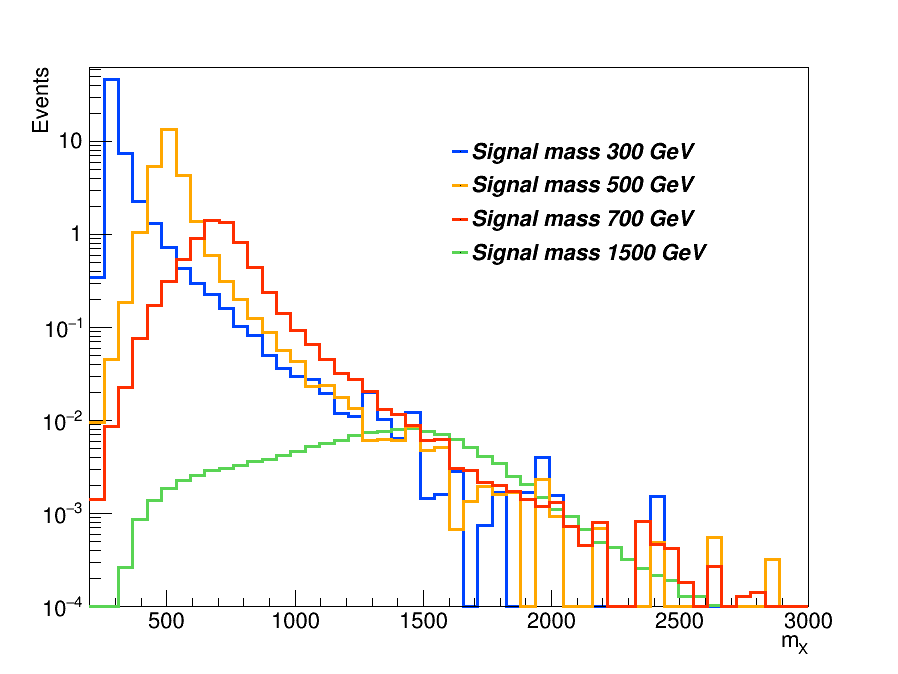
\includegraphics[width=0.45\textwidth]{../AN/Figs/Distribution_higgsLHEmass_cuts_nocuts.png}
}
\subfigure[$m_T^H$]{
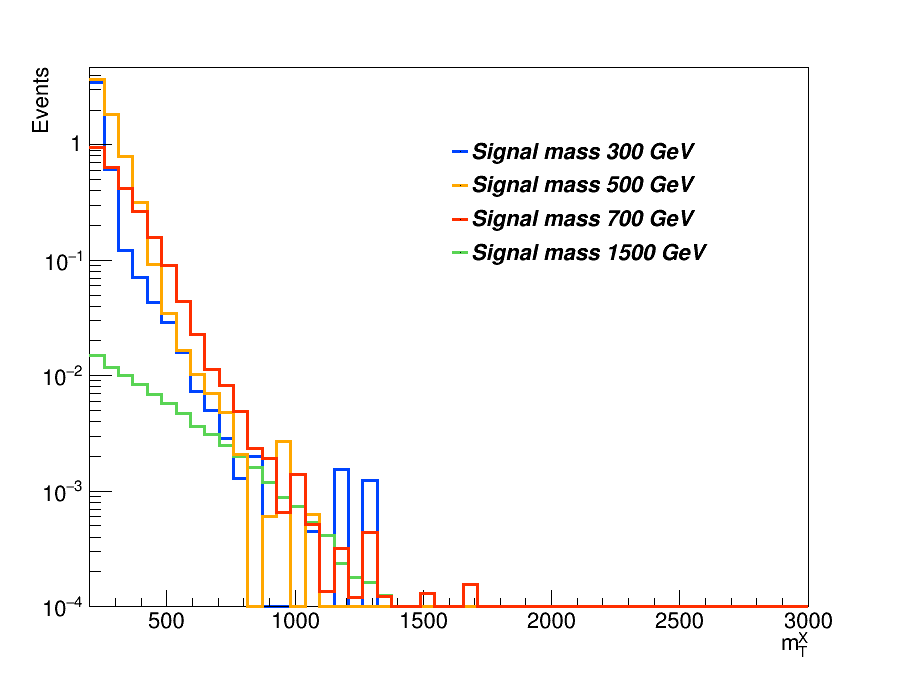
\includegraphics[width=0.45\textwidth]{../AN/Figs/Distribution_mth_cuts_nocuts.png}
}
\\
\subfigure[$m_{\ell \ell}$]{
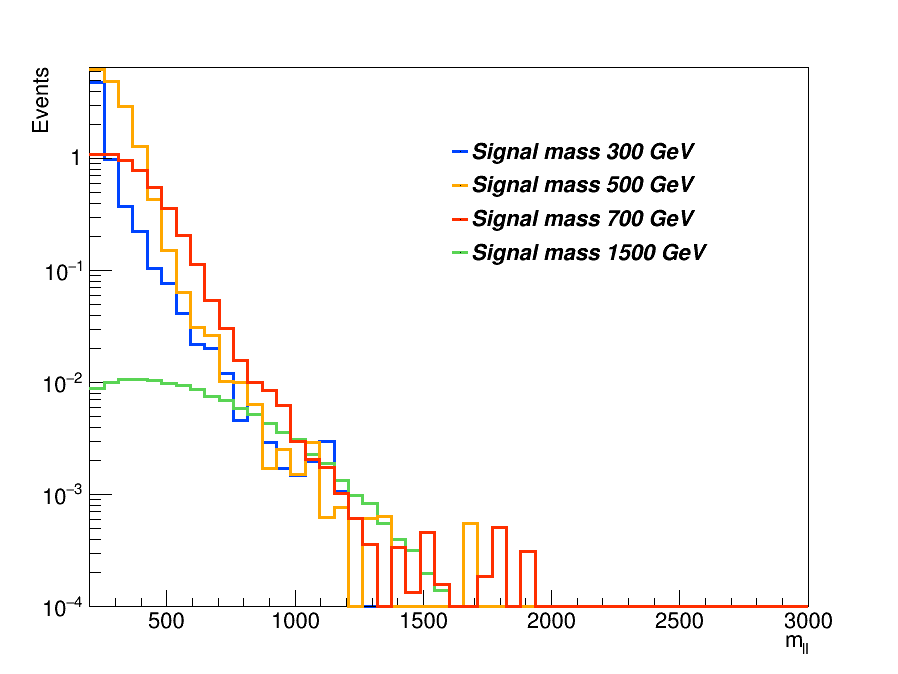
\includegraphics[width=0.45\textwidth]{../AN/Figs/Distribution_mll_cuts_nocuts.png}
}
\subfigure[$m_T^I$]{
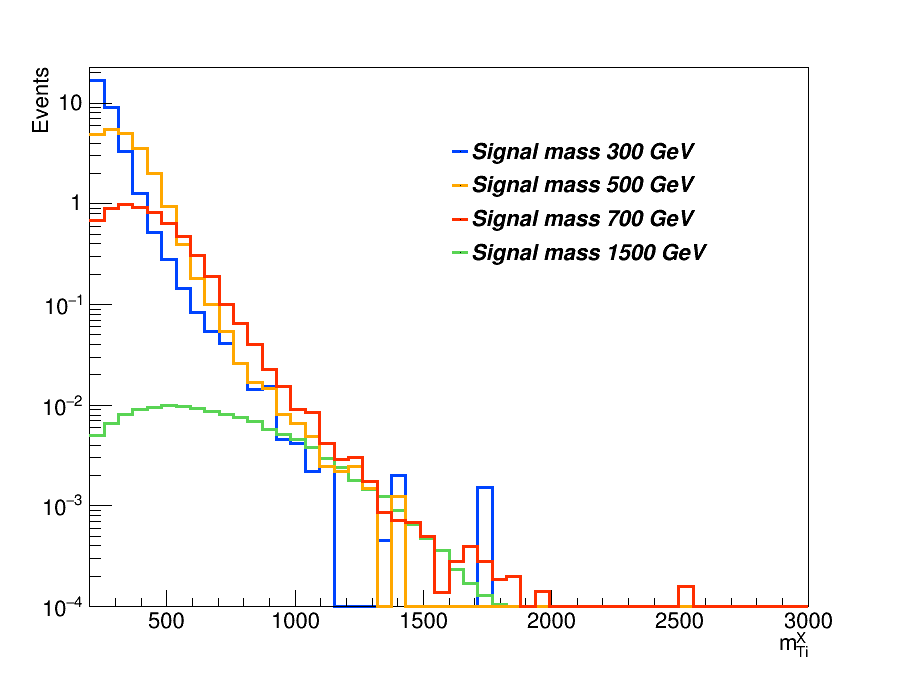
\includegraphics[width=0.45\textwidth]{../AN/Figs/Distribution_mTi_cuts_nocuts.png}
}
\caption{
    Distributions of the generated mass (no possible reconstruction), $m_T^H$, $m_{\ell \ell}$ and  $m_T^I$
    variables for different $X$ mass hypothesis. It is clear that the most discriminating variable is $m_T^I$. }
    \label{fig:mt_nocuts}
\end{figure}

%#################


\section{Signal interpretation: EW singlet, 2HDM and MSSM}
\label{sec:signalModel}
The signal is interpreted in terms of the electroweak singlet model, in 2HDM and finally in  MSSM model. The theory part of the models are described in Sec.~\ref{NSP}. 

\subsection*{Electroweak singlet model}
The EW singlet represents a scalar mixing among the high mass particle and the Higgs boson. This model relies on two parameters: the scale factor of the couplings of the high mass resonance with respect to the SM, $C'$, and the branching fraction of the electroweak singlet to non-SM decays modes, $BR_\mathrm{new}$. The electroweak singlet signal strength, $\mu'$ and the modified width, $\Gamma'$, are related with the parameters in the model by the following equations:
\begin{equation}
\mu' = C'^2 \cdot (1 - BR_\mathrm{new})
\end{equation}
\begin{equation}
\Gamma' = \Gamma_\mathrm{SM} \cdot \frac{C'^2}{1 - BR_\mathrm{new}}
\end{equation}
The high mass signal samples for different mass hypothesis have been reweighted according to this model. At the moment only the $BR_\mathrm{new} = 0$ hypothesis has been investigated while we tested different $C'$ values.
In Fig.~\ref{fig:cprime} are shown the \mll and \mt templates corresponding to a high mass boson  of 700\GeV for three different $C'$ values: $C' = 1$, corresponding to the SM Higgs decay width, $C'=0.5$, corresponding to $\Gamma' = 2.5\cdot10^{-2}\,\Gamma_\mathrm{SM}$, and $C'=0.1$, corresponding to $\Gamma' = 10^{-2}\,\Gamma_\mathrm{SM}$. A value of $BR_\mathrm{new} = 0$ is considered in all cases. We note that the signal shape is not very sensitive to different $C'$ values.
\begin{figure}[htbp]
\centering
\subfigure[Simulated LHE signals]{
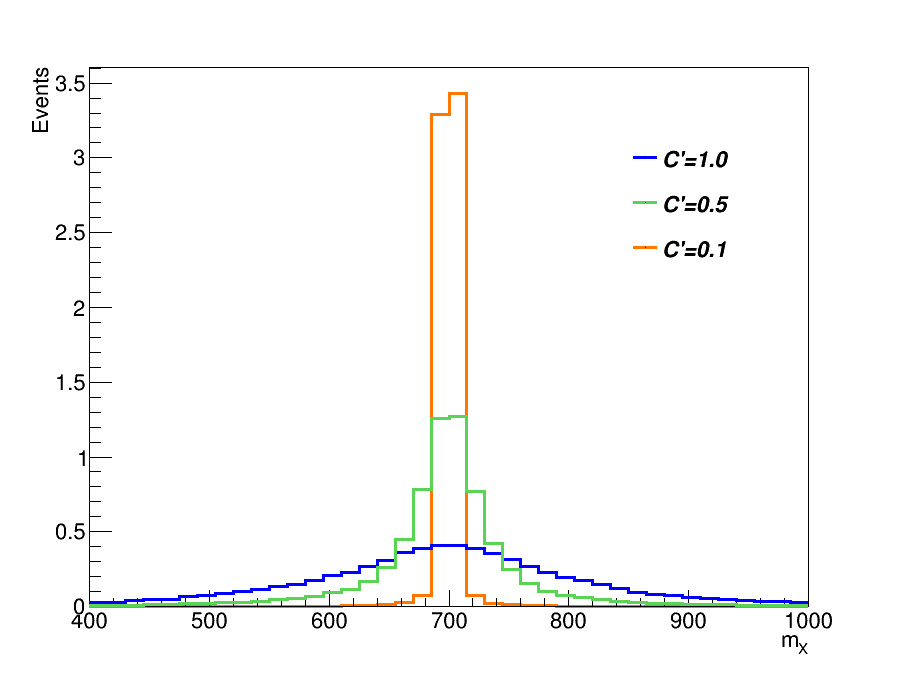
\includegraphics[width=0.45\textwidth]{../AN/Figs/higgsLHEmass700_cuts_nocuts.png}
}
\subfigure[$m_T^H$]{
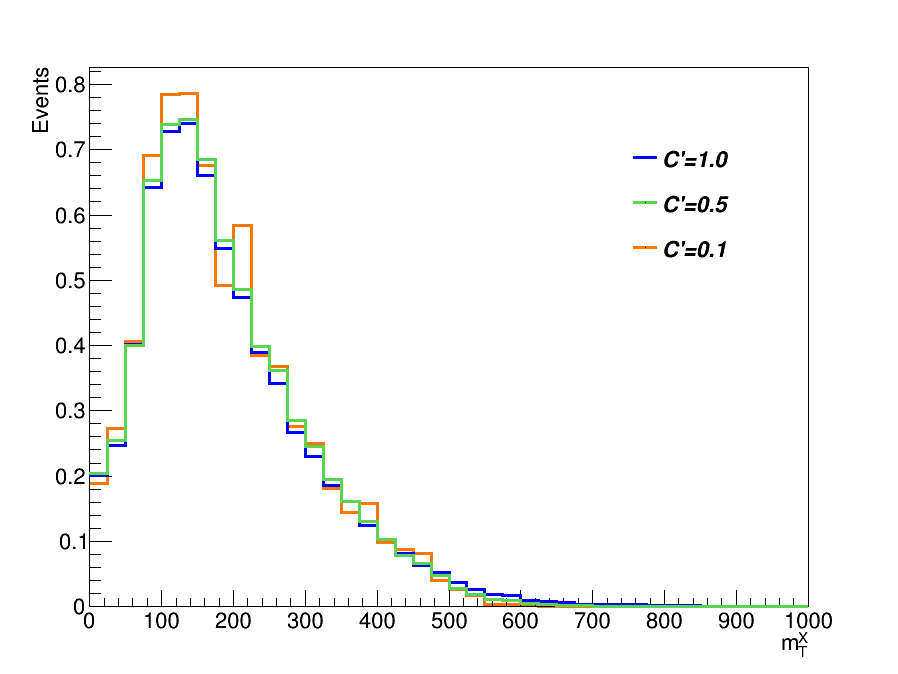
\includegraphics[width=0.45\textwidth]{../AN/Figs/mth700_cuts_nocuts.png}
}
\\
\subfigure[$m_{\ell \ell}$]{
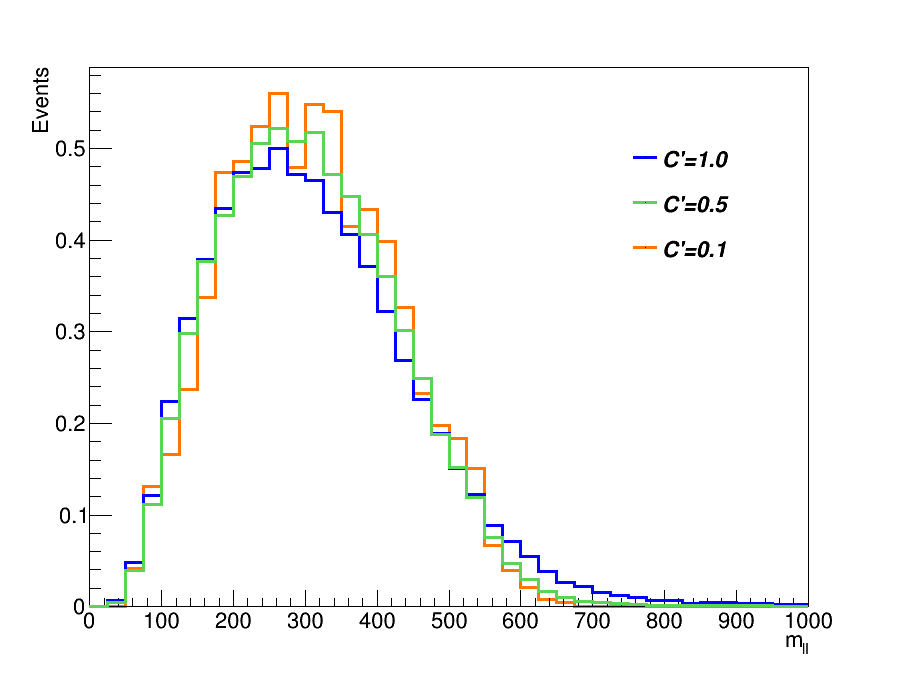
\includegraphics[width=0.45\textwidth]{../AN/Figs/mll700_cuts_nocuts.png}
}
\subfigure[$m_T^I$]{
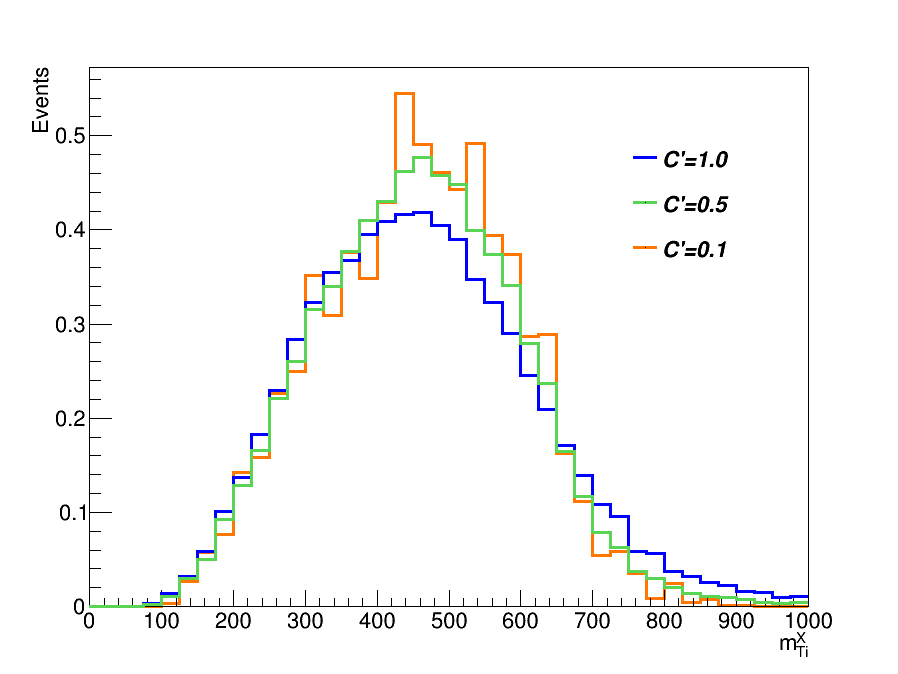
\includegraphics[width=0.45\textwidth]{../AN/Figs/mTi700_cuts_nocuts.png}
}
\caption{ 
    Distributions of the signals, the $m_T^H$, the $m_{\ell \ell}$ and the  $m_T^I$ variables at generator level for different values of $C'$, without any selection.}
    \label{fig:cprime}
\end{figure}

\subsection*{2HDM and MSSM models}
The 2HDM is a well motivated extension of the SM. It contains two Higgs doublets, from which a total of five Higgs bosons are predicted: Two CP-even bosons $h$ and $H$, a CP-odd boson $A$ and two charged bosons $H^\pm$. In most theories, $h$ exhibits the features of the SM Higgs boson, while $H$ is a CP-even Higgs boson at a higher mass. The 2HDM comprises many free parameters. Two of these are of particluar interest:
\begin{itemize}
\item $\tan\beta$: The ratio $\frac{v_u}{v_d}$ of the vacuum expectation values of the two Higgs doublets.
\item $\alpha$: The mixing angle of the two scalar Higgs bosons $h$ and $H$.
\end{itemize}
The quantity $\cos(\beta-\alpha)$ is also of interest, as the coupling of the heavy scalar Higgs boson $H$ to two vector bosons is proportional to this factor. In the decoupling limit, which occurs at $\cos(\beta-\alpha)=0$, all couplings become SM-like.
A 2HDM of type-2 is considered in this study. Here up-type quarks couple to one doublet, while down-type quarks and leptons couple to the other doublet.\\ 
\newline
The MSSM is a type-2 2HDM. On tree level only two parameters are left free. By convention, these parameters are chosen to be $\tan\beta$ and $m_{A}$, the mass of the pseudoscalar Higgs boson. The exclusion limits can be set in a two-dimensional plane as a function of these two parameters. Due to higher order diagrams additional free parameters occur. Benchmark scenarios are then used in order to constrain these parameters. Here two MSSM scenarios are used: the $m_{h}^{mod+}$ scenario and the hMSSM scenario \cite{Gori:2130983}.\\
\newline
The necessary model predictions for these scenarios are provided by the LHC Higgs Cross Section Working Group \cite{bsmhiggsxsecs}. For both MSSM scenarios the ggF cross sections have been computed with SusHi (v.1.4.1)\cite{Harlander:2012pb}. These cross sections include NLO supersymmetric QCD corrections and NNLO QCD corrections for the top quark contribution in the effective theory of a heavy top quark, as well as electroweak effects by light quarks. The masses of the Higgs bosons, their mixing, the branching fractions and the effective Yukawa couplings in the $m_{h}^{mod+}$ scenario are all calculated with FeynHiggs (v.2.10.2)\cite{Heinemeyer:1998yj, Heinemeyer:1998np, Degrassi:2002fi, Frank:2006yh, Hahn:2013ria}. For the hMSSM scenario the branching fractions are obtained from HDECAY (v.6.40)\cite{Djouadi:1997yw, Djouadi:2006bz}. The results for general 2HDM are obtained using the ggF cross sections computed with SusHi (v.1.5.0) and the branching fractions from 2HDMC (v.1.7.0)\cite{Rathsman:2011yv}. The VBF cross sections are calculated using an approximation. The BSM Higgs production cross sections for VBF, which are provided for different masses by the LHC Higgs Cross Section Working Group \cite{bsmhiggsxsecs2}, are taken and multiplied by $\cos^{2}(\beta-\alpha)$, resulting in VBF cross sections for a heavy CP-even Higgs boson.\newline
The exclusion limits obtained for the MSSM scenarios are displayed in the $m_{A}$-$\tan\beta$ plane. A fine grid is chosen in this plane, and for each point of this grid a maximum likelihood fit is performed after the $m_{A}$ and/or $\tan\beta$ dependent values of the model, such as cross sections and masses of the Higgs bosons are calculated. These fits are done using the asymptotic method. Performing a maximum likelihood fit in this manner is equivalent to a hypothesis test, where the signal hypothesis is tested against the SM-and-background hypothesis. The signal hypothesis for a combination of $m_{A}$ and $\tan\beta$ is excluded at $95\,\%$ confidence level. In the two-dimensional plane this limit is determined from interpolation between the points of the grid. The limits in the more general 2HDM are obtained in the same way, although a different parameter is chosen in place of $m_{A}$.


\section{Study of the Interference effects}
\label{sec:interference}
When a resonance $X$, with a non negligible width is considered, it is important to take into account also the interference effects both with the \WW background , with same initial and final state, and with the Higgs boson off-shell tail. 
In this analysis  the interference effects between the
new signal X produced in gluon-gluon fusion and in vector-boson-fusion is taken into account.
The effect of the various interference terms are shown in ~\ref{fig:X300} and  \ref{fig:Int_VBF_GEN} for the two different production mechanism, gluon-gluon fusion and vector-boson fusion.  The contribution of the interference of high mass resonances $X$ with the \WW background  and with the Higgs boson have opposite sign and partially cancel out. This cancellation effect is different for different resonance masses.
The interference contribution is thus non negligible and is included in the fit, Sec~\ref{StatIn}. \\
\begin{figure}[htbp]
\centering
\subfigure[Mass 300 \GeV.]{
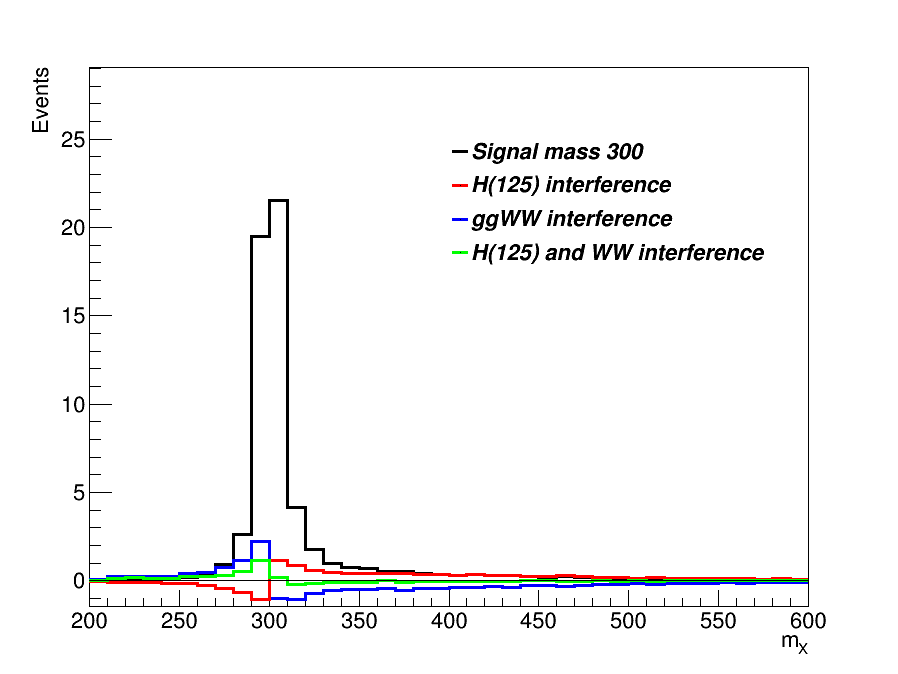
\includegraphics[width=0.45\textwidth]{../AN/Figs/Interference_higgsLHEmass300_cuts_nocuts.png}
}
\subfigure[Mass 400 \GeV.]{
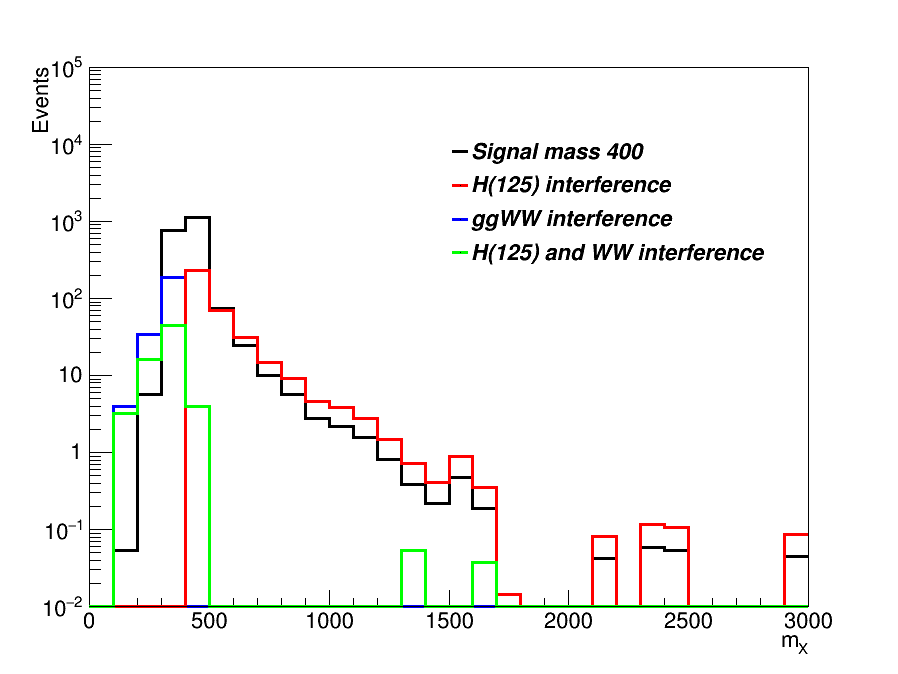
\includegraphics[width=0.45\textwidth]{../AN/Figs/Interference_higgsLHEmass400_cuts_nocuts.png}
}
\\
\subfigure[Mass 700 \GeV.]{
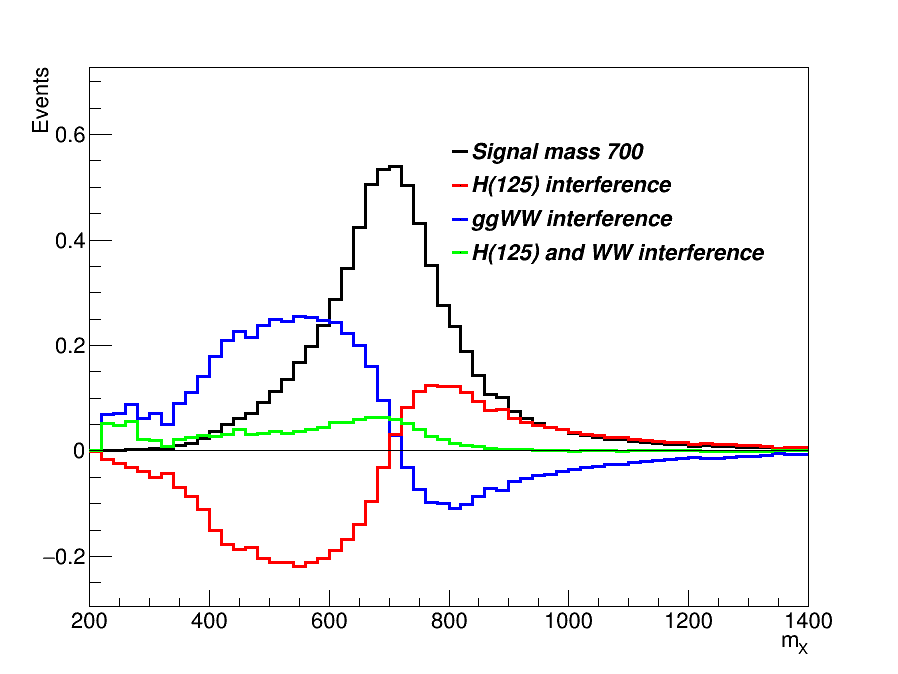
\includegraphics[width=0.45\textwidth]{../AN/Figs/Interference_higgsLHEmass700_cuts_nocuts.png}
}
\subfigure[Mass 1500 \GeV.]{
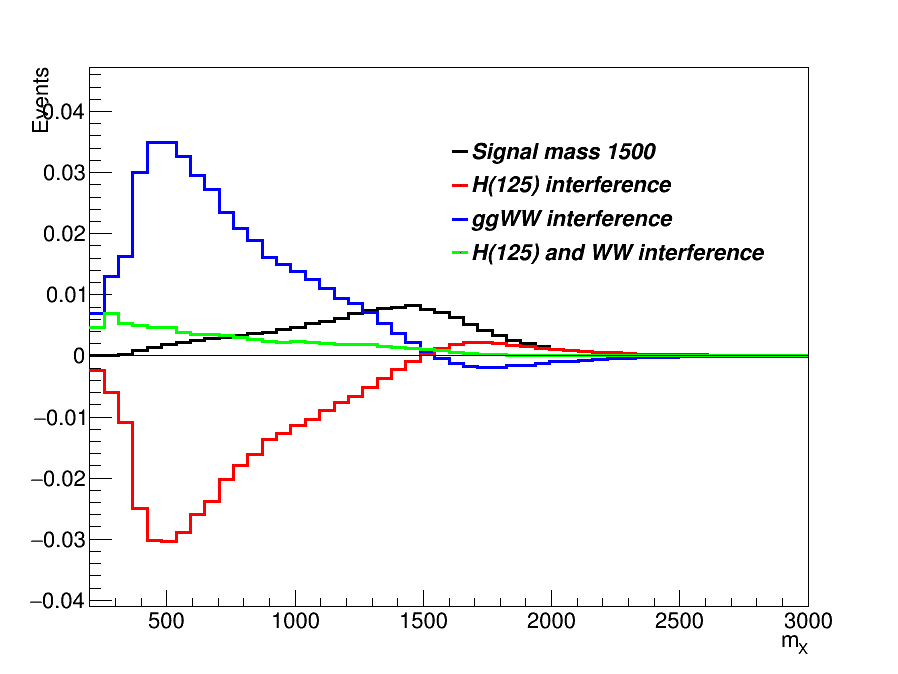
\includegraphics[width=0.45\textwidth]{../AN/Figs/Interference_higgsLHEmass1500_cuts_nocuts.png}
}
\caption{Distribution of for the $X$ mass resonance, produced via gluon-gluon fusion for different masses. In black the high mass signal. In red the interference between the high mass signal and the Higgs boson. In blue the interference between the high mass signal and the background. In green the total interference i.e. high 
mass signal, Higgs bison and background. }
    \label{fig:X300}
\end{figure}


\begin{figure}[htbp]
\centering
\subfigure[Mass 300 \GeV]{
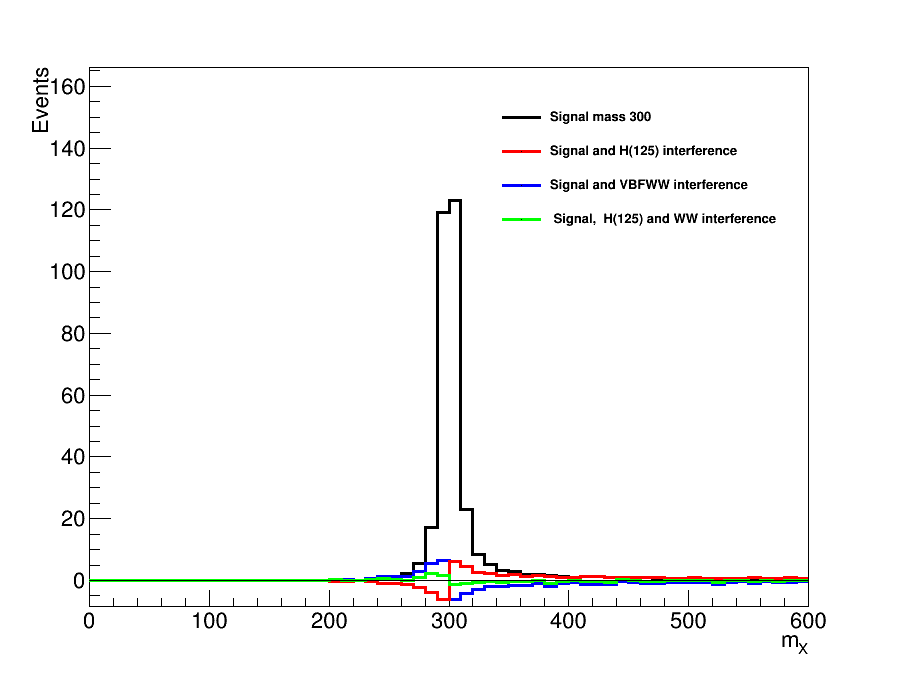
\includegraphics[width=0.45\textwidth]{../AN/Figs/Inter_VFB/Interference_higgsLHEmass300_cuts_nocuts.png}
}
\subfigure[Mass 1500 \GeV]{
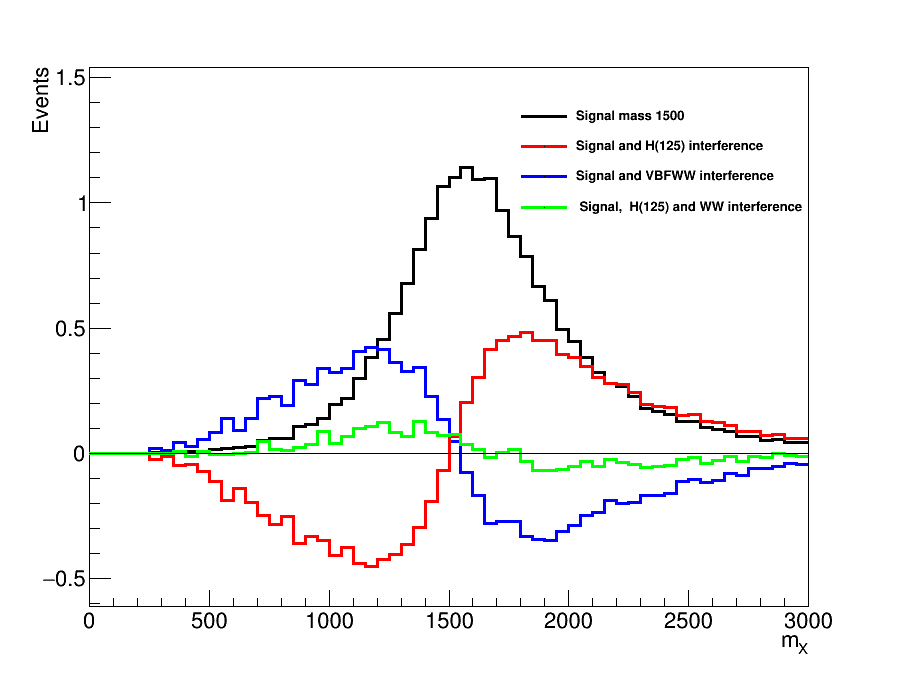
\includegraphics[width=0.45\textwidth]{../AN/Figs/Inter_VFB/Interference_higgsLHEmass1500_cuts_nocuts.png}
}
\caption{Distribution of for the $X$ mass resonance, produced via vector-boson-fusion fusion for different masses. In black the high mass signal. In red the interference between the high mass signal and the Higgs boson. In blue the interference between the high mass signal and the background. In green the total interference i.e. high 
mass signal, Higgs bison and background.}
    \label{fig:Int_VBF_GEN}
\end{figure}


\section{Main Background}
